%
%  version 1, 2016-12-05
%
\documentclass[twocolumn,twoside]{svmultivs_br} %please do not change this line
\usepackage{graphicx}
%
% The contents of \title* are printed on the first page.
% The contents of \subtitle are printed below the title on the
% first page.  This keyword is optional.
% The contents of \titlerunning are printed on the other pages.
% This should be a short version of the title.
%
\title*{Your Title}
%\subtitle{Optional Sub-title on first page}
\titlerunning{Short Version of Your Title}
%
% Example:
% \title*{IVS Coordinating Center 2019--2020 Biennial Report}
% \titlerunning{IVS CC 2019--2020 Report}
%
% \subtitle may be used if there is not enough room in \title*.  
% Example:
% \title*{International VLBI Service Coordinating Center Biennial Report Submission}
% \subtitle{Work during 2019--2020}
% \titlerunning{IVS CC 2019--2020 Report}
%
\author{Name of First Author$^1$, Name of Second Author$^{1,2}$, Name of Third Author$^3$}
\authorrunning{Last Name(s) of Author(s)} % see comments below
\authoremails{e-mail address of first author, e-mail address of second author, e-mail address of third author}
\institute{1. Institution Name 1 \\ 2. Institution Name 2 \\ 3. Institution Name 3}
%
% \author and \institute keywords:
%
% Each number in \author refers to an institution with which the author is associated.
% The numbers should correspond to numbered institutions in the \institute keyword.
% If all authors are associated with only one institution (the same institution),
% then the numbers should be omitted from \author and \institute.
% If an author is associated with two or more institutions, multiple numbers may be
% used.
%
% The \institute key word must be a single line.
% Please separate institutions using \\ between each institution.
%
% \authorrunning keyword:
%
% For one author, please use \authorrunning{last_name_of_author},
% e.g., \authorrunning{Behrend}
% For two authors, please use \authorrunning{last_name_of_first_author and last_name_of_second_author}
% e.g., \authorrunning{Behrend and Baver}
% For three or more authors, please use \authorrunning{last_name_of_first_author et al.}
% e.g., \authorrunning{Behrend et al.}
%
% Examples
%
% \author{Dirk Behrend}
% \authorrunning{Behrend}
% \author_emails{dirk.behrend-1@nasa.gov}
% \institute{NVI, Inc.}
%
% \author{Karen Baver, Dirk Behrend}
% \authorrunning{Baver and Behrend}
% \author_emails{karen.d.baver@nasa.gov,dirk.behrend-1@nasa.gov}
% \institute{NVI, Inc.}
%
% \author{John Gipson~$^1$, David Eriksson~$^{1,2}$, Chopo Ma~$^3$}
% \authorrunning{Gipson et al.}
% \institute{1. NVI, Inc. \\ 2. Chalmers University of Technology \\ 3. Goddard Space Flight Center}
%
\component{Short-component-identifier  Component-type} 
%
% Examples:
%    Mets\"ahovi Network Station
%    NEOS Operation Center
%    Bonn Correlator
%    INAF Data Center
%    IAA Analysis Center
%    NICT Technology Development Center
%
% Exceptions are the coordinators, who should use
%    IVS Analysis Coordinator
% etc.
%    
% \ContactAuthorName, \ContactAuthorTelephone, and \ContactAuthorEmail 
% should be used to identify the preferred contact author.
%
\ContactAuthorName{Name of Contact Author}
\ContactAuthorTelephone{Phone Number}
\ContactAuthorEmail{E-mail Address}
%
\NumberofInstitutions{2}
\InstitutionPostAddress{1}{Address part 1a, Address part 1b, Address part 1c}
\InstitutionCountry{1}{Country 1}
\InstitutionWebPage{1}{Web Address 1}
\InstitutionPostAddress{2}{Address part 2a, Address part 2b, Address part 2c, Address part 2d}
\InstitutionCountry{2}{Country 2}
\InstitutionWebPage{2}{Web Address 2}
%
% Example:
%
% \InstitutionPostAddress{1}{61 avenue de l'Observatoire, 75014 Paris}
% \InstitutionCountry{1}{France}
% \InstitutionWebPage{1}{http://www.obspm.fr}
%
\begin{document}  %please do not change this line
%
\maketitle       %please do not change this line
%
\abstract{Please insert abstract here.}
%
\section{General Information}
%
Please insert text.
%
\section{Activities during the Past Year}
%
Please insert text.
%
\section{Current Status}
%
Please insert text.
%
\section{Future Plans}
%
Please insert text.
%
% Code to include a single column figure through \includegraphics.
% \begin{figure} and \end{figure} make this single column.
% If the figure is too wide, it will overwrite text in the other column.
% Figures should be centered through the latex \begin{center} and
% \end{center} commands.  
% Captions should be left-justified.  
% The class file will automatically perform the left-justification,
% if the caption is not included in the latex centering.
%
\begin{figure}[htb!]         
  \begin{center}
%
% Please specify the file extension as part of the figure
% file name. The formats of jpg, png and pdf can be used.
% Sample files names are: 
%       acgsfc01.jpg  
%       tdgsfc01.png and tdgsfc02.png
%       occore01.jpg, occore02.png, and occore03.pdf.
%
  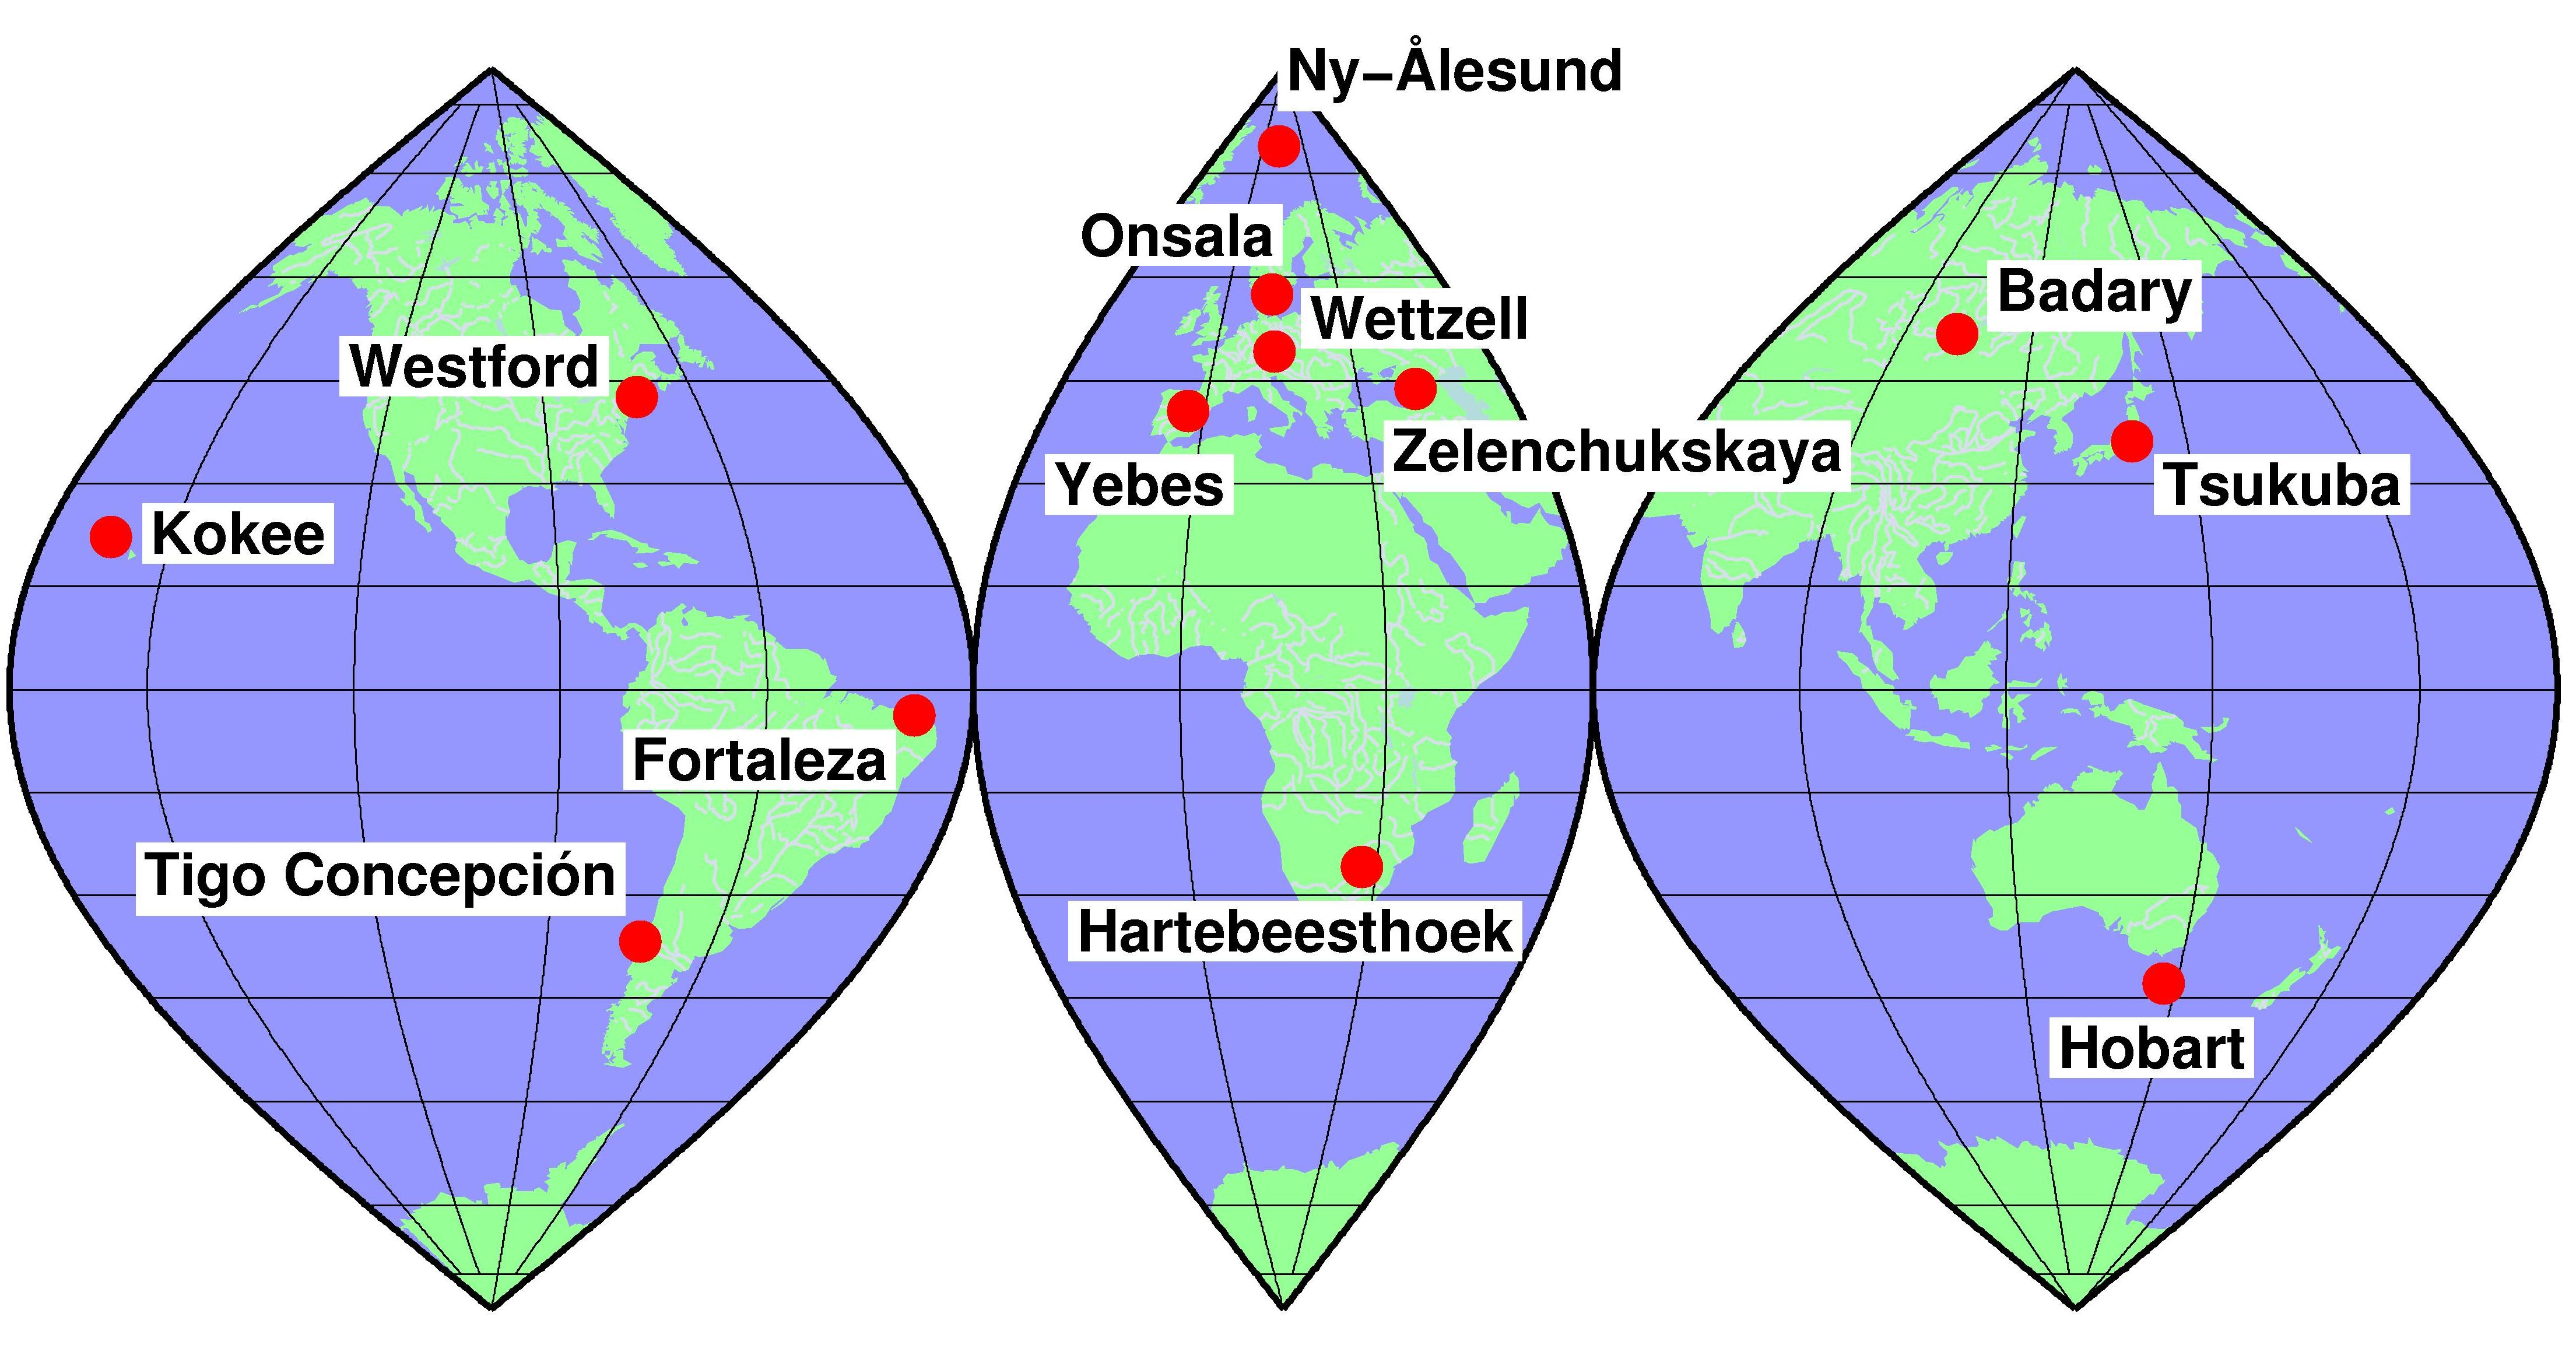
\includegraphics[width=.5\textwidth]{ivs-br-template01.jpg}
%%%%%  The caption should not be preceded by Figure 1.  
%%%%%  Please just enter your desired caption, such as:
%%%%%         Equipment at our station.
  \end{center}
  \caption{Example of figure from .jpg file.}
  \label{first-unique-label}             
\end{figure}                     
%
% Code to use \includegraphics to include a figure that spans two columns. 
% \begin{figure*} and \end{figure*} will allow the figure to Span 
% two columns.  If the figure is too narrow, it will leave blank space 
% in the other column.
% Figures should be centered through the latex \begin{center} and
% \end{center} commands.  
% Captions should be left-justified.  
% The class file will automatically perform the left-justification,
% if the caption is not included in the latex centering.
%
\begin{figure*}[htb!]
% Please see the above figure example for naming conventions for the 
% figure file.
\begin{center}
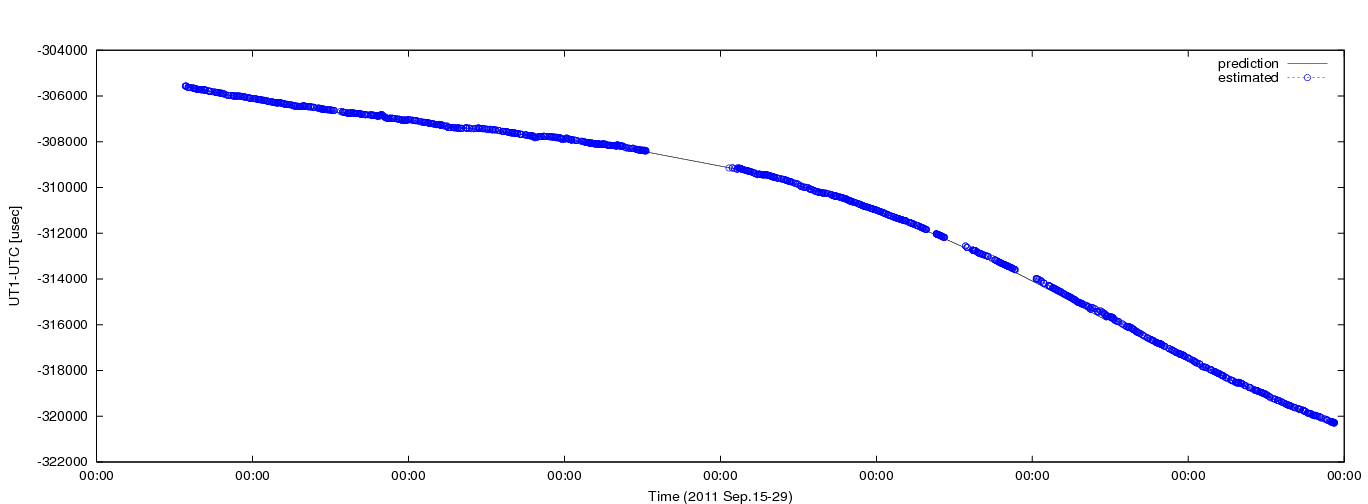
\includegraphics[width=16.0cm]{ivs-br-template02.png}
\end{center}
% Please do not precede the caption by Figure 2.  
% Please just enter your desired text.
\caption{Example of figure from .png file.}
\label{second-unique-label}
\end{figure*}
%
% Code to include a single column table.
% Other table formats may be used also.  
% Tables should be centered through the latex \begin{center} and
% \end{center} commands.  
% Captions should be left-justified.  
% The class file will automatically perform the left-justification,
% if the caption is not included in the latex centering.
%
\begin{table}[htb!]
\caption{Caption for Table 1.}
\begin{center}
\begin{tabular}{|l|c|c|r|} \hline
Heading 1 & Heading 2 & Heading 3 & Heading 4\\
\hline
Value a1 & Value a2 & Value a3 &          \\
Value b1 &          & Value b3 & Value b4 \\
Value c1 & Value c2 & Value c3 &          \\
Value d1 & Value d2 & Value d3 & Value d4 \\
Value e1 & Value e2 & Value e3 & Value e4 \\
\hline
\end{tabular}
\end{center}
\label{third-unique-label}
\end{table}
%
% Code to include a two column table.
% Other table formats may be used also.  
% Tables should be centered through the latex \begin{center} and
% \end{center} commands.  
% Captions should be left-justified.  
% The class file will automatically perform the left-justification,
% if the caption is not included in the latex centering.
%
\begin{table*}[htb!]
\caption{Caption for Table 2.}
\begin{center}
\begin{tabular}{|l|c|c|r|l|c|c|r|} \hline
Heading 1 & Heading 2 & Heading 3 & Heading 4 & Heading 5 & Heading 6 & Heading 7 & Heading 8\\
\hline
Value a1 & Value a2 & Value a3 &          & Value a5 & Value a6 & Value a7 & Value a8 \\
Value b1 &          & Value b3 & Value b4 &          &          & Value b7 & Value b8 \\
Value c1 & Value c2 & Value c3 &          & Value c5 & Value c6 & Value c7 &          \\
Value d1 & Value d2 & Value d3 & Value d4 & Value d5 & Value d6 &          &          \\
Value e1 & Value e2 & Value e3 & Value e4 & Value e5 &          & Value e7 &          \\
Value f1 & Value f2 & Value f3 & Value f4 & Value f5 &          & Value f7 &          \\
Value g1 &          & Value g3 & Value g4 & Value g5 & Value g6 & Value g7 & Value g8 \\
\hline
Value h1 & Value h2 & Value h3 &          & Value h5 & Value h6 & Value h7 & Value h8 \\
Value i1 &          & Value i3 & Value i4 &          &          & Value i7 & Value i8 \\
Value j1 & Value j2 & Value j3 &          & Value j5 & Value j6 & Value j7 &          \\
Value k1 & Value k2 & Value k3 & Value k4 & Value k5 & Value k6 &          &          \\
Value l1 & Value l2 & Value l3 & Value l4 & Value l5 &          & Value l7 &          \\
Value m1 & Value m2 & Value m3 & Value m4 & Value m5 &          & Value m7 &          \\
Value n1 &          & Value n3 & Value n4 & Value n5 & Value n6 & Value n7 & Value n8 \\
\hline
Value o1 & Value o2 & Value o3 &          & Value o5 & Value o6 & Value o7 & Value o8 \\
Value p1 &          & Value p3 & Value p4 &          &          & Value p7 & Value p8 \\
Value q1 & Value q2 & Value q3 &          & Value q5 & Value q6 & Value q7 &          \\
Value r1 & Value r2 & Value r3 & Value r4 & Value r5 & Value r6 &          &          \\
Value s1 & Value s2 & Value s3 & Value s4 & Value s5 &          & Value s7 &          \\
Value t1 & Value t2 & Value t3 & Value t4 & Value t5 &          & Value t7 &          \\
Value u1 &          & Value u3 & Value u4 & Value u5 & Value u6 & Value u7 & Value u8 \\
\hline
Value v1 & Value v2 & Value v3 &          & Value v5 & Value v6 & Value v7 & Value v8 \\
Value w1 &          & Value w3 & Value w4 &          &          & Value w7 & Value w8 \\
Value x1 & Value x2 & Value x3 &          & Value x5 & Value x6 & Value x7 &          \\
Value y1 & Value y2 & Value y3 & Value y4 & Value y5 & Value y6 &          &          \\
Value z1 & Value z2 & Value z3 & Value z4 & Value z5 &          & Value z7 &          \\
\hline
\end{tabular}
\end{center}
\label{fourth-unique-label}
\end{table*}
%
% Please see the first two figures for detailed information
% about using figures.
%
\begin{figure*}[htb!]
\begin{center}
\includegraphics[width=16.0cm]{ivs-br-template03.pdf}
\end{center}
\caption{Example of figure from .pdf file.}
\label{fifth-unique-label}
\end{figure*}
%
% The acknowledgements section is optional.  If used, the section line should 
% be:
%      \section*{Acknowledgements}
%
\section*{Acknowledgements}

This section is optional.
%
% The bibliography section is optional.
%
% Here is a section with some examples.
% But the entries are free-format --- essentially,
%  \bibitem{unique-label}
%  text
%
%%%%%\begin{thebibliography}{99}
%%%%%\bibitem{Abbondanza2012}
%%%%%C.~Abbondanza and P.~Sarti.
%%%%%Impact of network geometry, observation schemes and telescope structure deformations on local ties:
%%%%%simulations applied to Sardinia Radio Telescope.
%%%%%\emph{Journal of Geodesy}, 86(3), doi:10.1007/s00190-011-0507-6, 181--192, 2012.
%%
%%%%%\bibitem{Artz}
%%%%%Thomas Artz, Judith Leek, Axel Nothnagel, and Maike Schumacher.
%%%%%VLBI Intensive Sessions Revisited.
%%%%%In D.~Behrend and K.~Baver, editors, \emph{International
%%%%%  VLBI Service for Geodesy and Astrometry 2012 General Meeting Proceedings},
%%%%%  NASA/CP-2012-217504, pages 276--280, 2012.
%%%%%%%
%%%%%\bibitem{VieVS}
%%%%%Matthias Madzak, Sigrid B\"ohm, Hana Kr\'asn\'a, and Lucia Plank.
%%%%%Vienna VLBI Software Version 2.1 User Manual
%%%%%Web document http://vievs.geo.tuwien.ac.at/fileadmin/editors/VieVS/documents/vievsDoc.pdf
%%%%%%
%%%%%\end{thebibliography} 
\begin{thebibliography}{99}

\bibitem{IVS-CC}
D.~Behrend, ``Coordinating Center Report'',
In K.\ D.\ Baver, D.\ Behrend, and K.\ Armstrong, editors, International
VLBI Service for Geodesy and Astrometry 2012 Annual Report,
NASA/TP-2013-217511, pages 55--57, 2013.

\end{thebibliography}
%
\end{document}
